\begin{center}
\Huge
	Inverse funktioner 
\end{center}
\section*{Inverse funktioner}
\stepcounter{section}
Vi husker på fra sidst at inverse funktioner defineres på følgende vis. 
\begin{defn}[Invers funktion]
	For en funktion $f:A\to B$ siges en funktion $g:B\to A$ at være \textit{invers funktion} til $g$, hvis det gælder, 
	at 
	\begin{align*}
		f\circ g (x) = x
	\end{align*}
	og
	\begin{align*}
		g \circ f(x) = x.
	\end{align*}
	I så fald skriver vi $g = f^{-1}$.
\end{defn}

Vi har følgende forhold mellem inverse funktioner og bijektive funktioner.
\begin{setn}
	En funktion $f$ har en invers funktion hvis og kun hvis den er bijektiv. 
\end{setn}
Intuitivt nok er det klart, at en funktion skal være bijektiv for at have en invers funktion. Ellers er det svært at forestille sig en veldefineret funktion på hele dispositionsmængden.

\begin{exa}
	Funktionen $f:\mathbb{R} \to \mathbb{R}$ givet ved 
	\begin{align*}
		f(x) = x^2
	\end{align*}
	er ikke hverken injektiv eller surjektiv. For at finde dens inverse funktion ændrer vi derfor på
	definitions- og dispositionsmængden, så $f$ i stedet defineres på $f:\mathbb{R}_{\geq 0} \to 
	\mathbb{R}_{\geq 0}$. Så har vi den inverse funktion til $f$ givet ved
	\begin{align*}
		f^{-1}(x) = \sqrt{x},
	\end{align*}
	altså kvadratrodsfunktionen. 
\end{exa}

Vi kan se en illustration af en invers funktion på Figur \ref{fig:inv}. 
\begin{figure}[H]
	\centering
	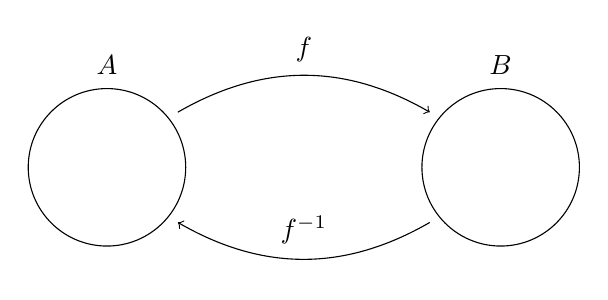
\begin{tikzpicture}
		\draw (0,0) circle (1cm);
		\draw (5,0) circle (1cm);
		\draw[-{To[scale = 1.3]}] (0.9,0.7)	to[out = 30, in = 150] (4.1,0.7);
		\draw[-{To[scale = 1.3]}] (4.1,-0.7)	to[out = -150, in = -30] (0.9,-0.7);
		\node at (0,1.3) {$A$};
		\node at (5,1.3) {$B$};
		\node at (2.5,1.5) {$f$};
		\node at (2.5,-0.8) {$f^{-1}$};
	\end{tikzpicture}
	\caption{Funktion $f$ samt invers funktion $f^{-1}$.}
	\label{fig:inv}
\end{figure}

\begin{exa}
	Skal vi finde inverse funktioner til bijektive funktioner, så skal vi altid isolere $x$ i forskriften for 
	funktionen. Vi betragter følgende funktion $f$ givet ved
	\begin{align*}
		f(x) = 5^{7x-11}.
	\end{align*}
	Vi sætter $y = f(x)$ og isolerer.
	\begin{align*}
		y = 5^{7x-11} \ &\Leftrightarrow \ \log_5(y) = 5^{7x-11} = 7x-11 \\
		&\Leftrightarrow	 \ \log_5(y)+11 = 7x \\
		&\Leftrightarrow	 \ \frac{\log_5(y)+11}{7} = x.
	\end{align*}
	Den inverse funktion til $f$ lyder derfor
	\begin{align*}
		f^{-1}(x) = \frac{\log_5(x) + 11}{7}.
	\end{align*}
\end{exa}

\section*{Grafer for inverse funktioner}
\stepcounter{section}

Når vi skal tegne grafer for inverse funktioner, så skal vi spejle grafen for $f$ i linjen $y = x$. En illustration af dette kan ses på Figur \ref{fig:invgraf} for funktionerne $f(x) = x^2$ og $f^{-1}(x) = \sqrt{x}$.

\begin{figure}[H]
	\centering
	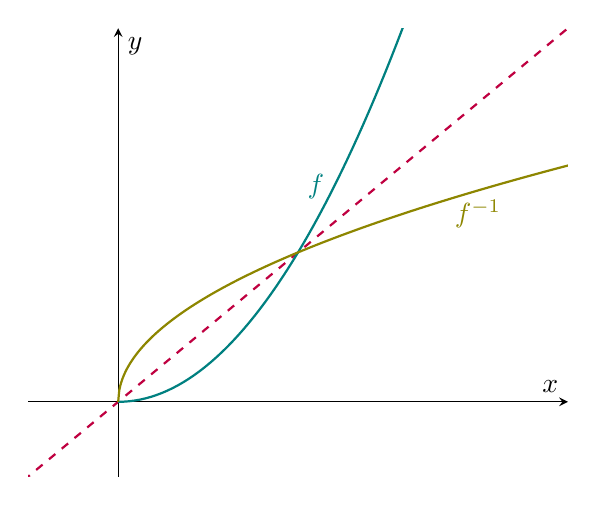
\begin{tikzpicture}
	\begin{axis}[
	axis lines = center, 
	xmin = -0.5, xmax = 2.5,
	ymin = -0.5, ymax = 2.5,
	ticks = none, 
	xlabel = $x$, 
	ylabel = $y$,
	]
		\addplot[color = purple, thick, dashed] {x};
		\addplot[color = teal, thick, samples = 100, domain = 0:3] {x^2};
		\addplot[color = olive, thick, samples = 500, domain = 0:3] {sqrt(x)};
		\node[color = teal, anchor = east] at (axis cs: 1.2,1.44) {$f$};
		\node[color = olive, anchor = north] at (axis cs: 2, 1.4142) {$f^{-1}$};
	\end{axis}
	\end{tikzpicture}
	\caption{Grafer for $f$ og $f^{-1}$.}
	\label{fig:invgraf}
\end{figure}

Den inverse funktion til eksponentialfunktioner er logaritmefunktioner. På Figur \ref{fig:invgraflog} kan vi se 
den inverse funktion til $2^x$. 
\begin{figure}[H]
	\centering
	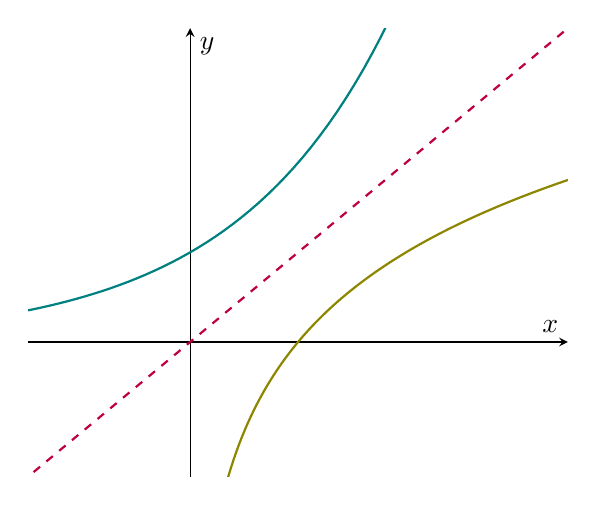
\begin{tikzpicture}
	\begin{axis}[
	axis lines = center, 
	xmin = -1.5, xmax = 3.5,
	ymin = -1.5, ymax = 3.5,
	ticks = none, 
	xlabel = $x$, 
	ylabel = $y$,
	]
		\addplot[color = purple, thick, dashed] {x};
		\addplot[color = teal, thick, samples = 100, domain = -3:5] {2^x};
		\addplot[color = olive, thick, samples = 500, domain = 0:5] {ln(x)/ln(2)};
	\end{axis}
	\end{tikzpicture}
	\caption{Grafer for $2^x$ og $\log_{2}(x)$.}
	\label{fig:invgraflog}
\end{figure}

\newpage
\subsection*{Opgave 1}
Tegn inverse funktioner for funktionerne givet ved følgende grafer.
\begin{center}
	\resizebox{0.45\textwidth}{!}{
	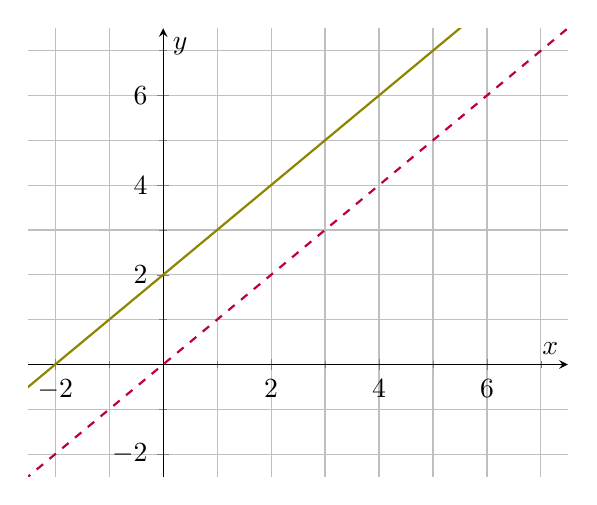
\begin{tikzpicture}
	\begin{axis}[
	axis lines = center, 
	xmin = -2.5, xmax = 7.5,
	ymin = -2.5, ymax = 7.5,
	xlabel = $x$, 
	ylabel = $y$,
	xtick = {-4,-2,...,6,8},
	ytick = {-4,-2,...,6,8},
	minor tick num = 1,
	grid = both,
	]
		\addplot[color = purple, thick, dashed, domain = -4:10] {x};
		\addplot[color = olive, thick, samples = 100, domain = -4:10] {x+2};
	\end{axis}
	\end{tikzpicture}
	}
	\resizebox{0.45\textwidth}{!}{
	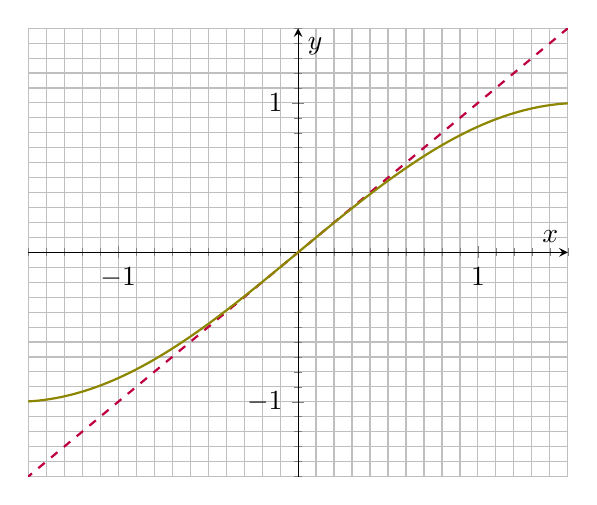
\begin{tikzpicture}
	\begin{axis}[
	axis lines = center, 
	xmin = -1.5, xmax = 1.5,
	ymin = -1.5, ymax = 1.5,
	xlabel = $x$, 
	ylabel = $y$,
	xtick = {-2,-1,...,3,4},
	ytick = {-2,-1,...,3,4},
	minor tick num = 9,
	grid = both,
	]
		\addplot[color = purple, thick, dashed, domain = -4:10] {x};
		\addplot[color = olive, thick, samples = 100, domain = -1.57:1.57] {sin(deg(x))};
	\end{axis}
	\end{tikzpicture}
	}
	
	\resizebox{0.45\textwidth}{!}{
	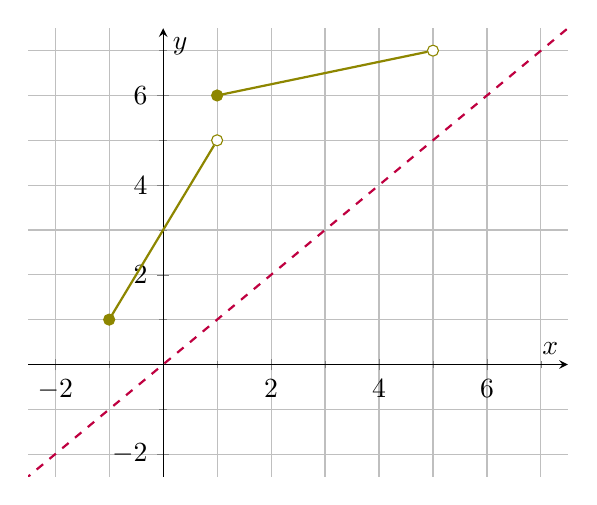
\begin{tikzpicture}
	\begin{axis}[
	axis lines = center, 
	xmin = -2.5, xmax = 7.5,
	ymin = -2.5, ymax = 7.5,
	xlabel = $x$, 
	ylabel = $y$,
	xtick = {-4,-2,...,6,8},
	ytick = {-4,-2,...,6,8},
	minor tick num = 1,
	grid = both,
	]
		\addplot[color = purple, thick, dashed, domain = -4:10] {x};
		\addplot[color = olive, thick, samples = 100, domain = -1:1] {2*x+3};
		\filldraw[color = olive] (axis cs: -1,1) circle (2pt);
		\filldraw[color = white] (axis cs: 1,5) circle (2pt);
		\draw[color = olive] (axis cs: 1,5) circle (2pt);
		\addplot[color = olive, thick, samples = 100, domain = 1:5] {0.25*x+5.75};
		\filldraw[color = olive] (axis cs: 1,6) circle (2pt);
		\filldraw[color = white] (axis cs: 5,7) circle (2pt);
		\draw[color = olive] (axis cs: 5,7) circle (2pt);
	\end{axis}
	\end{tikzpicture}
	}
	\resizebox{0.45\textwidth}{!}{
	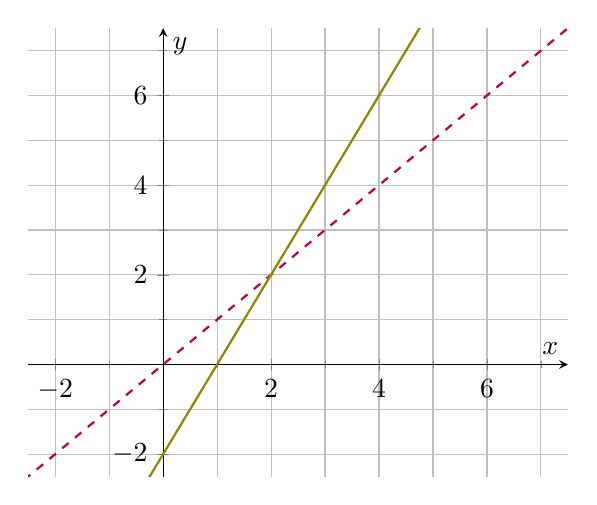
\begin{tikzpicture}
	\begin{axis}[
	axis lines = center, 
	xmin = -2.5, xmax = 7.5,
	ymin = -2.5, ymax = 7.5,
	xlabel = $x$, 
	ylabel = $y$,
	xtick = {-4,-2,...,6,8},
	ytick = {-4,-2,...,6,8},
	minor tick num = 1,
	grid = both,
	]
		\addplot[color = purple, thick, dashed, domain = -4:10] {x};
		\addplot[color = olive, thick, samples = 100, domain = -4:10] {2*x-2};
	\end{axis}
	\end{tikzpicture}
	}
	\resizebox{0.45\textwidth}{!}{
	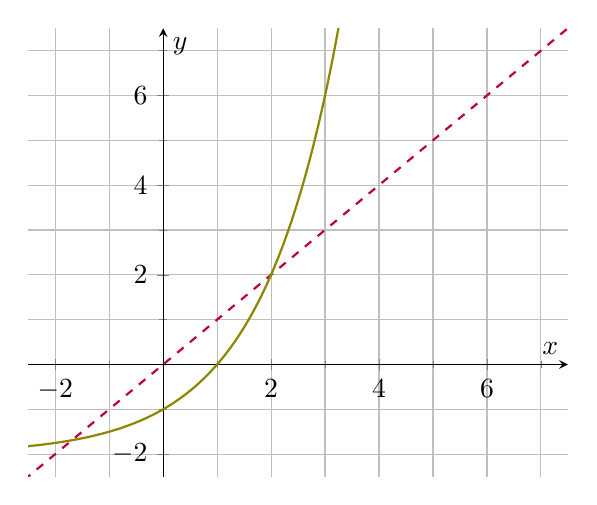
\begin{tikzpicture}
	\begin{axis}[
	axis lines = center, 
	xmin = -2.5, xmax = 7.5,
	ymin = -2.5, ymax = 7.5,
	xlabel = $x$, 
	ylabel = $y$,
	xtick = {-4,-2,...,6,8},
	ytick = {-4,-2,...,6,8},
	minor tick num = 1,
	grid = both,
	]
		\addplot[color = purple, thick, dashed, domain = -4:10] {x};
		\addplot[color = olive, thick, samples = 100, domain = -4:4] {2^x - 2};
	\end{axis}
	\end{tikzpicture}
	}
	\resizebox{0.45\textwidth}{!}{
	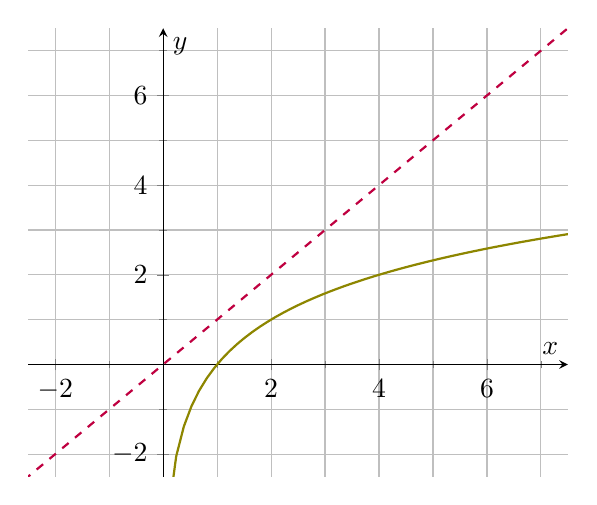
\begin{tikzpicture}
	\begin{axis}[
	axis lines = center, 
	xmin = -2.5, xmax = 7.5,
	ymin = -2.5, ymax = 7.5,
	xlabel = $x$, 
	ylabel = $y$,
	xtick = {-4,-2,...,6,8},
	ytick = {-4,-2,...,6,8},
	minor tick num = 1,
	grid = both,
	]
		\addplot[color = purple, thick, dashed, domain = -4:10] {x};
		\addplot[color = olive, thick, samples = 100, domain = -4:10] {ln(x)/ln(2)};
	\end{axis}
	\end{tikzpicture}
	}
\end{center}

\newpage


\subsection*{Opgave 2}
En funktion $f$ er givet ved følgende graf.
\begin{center}
\resizebox{0.45\textwidth}{!}{
	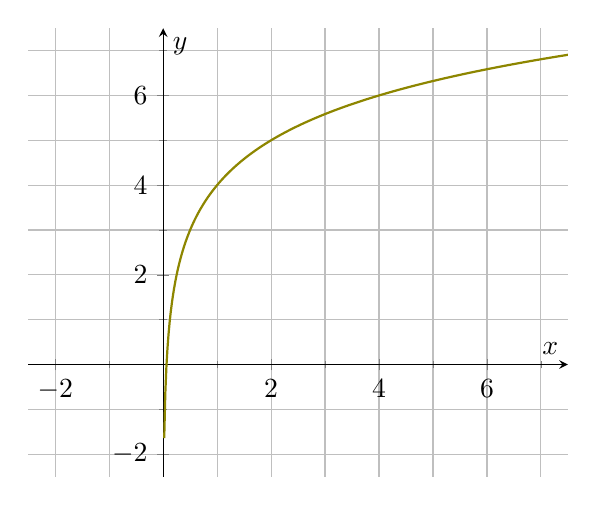
\begin{tikzpicture}
	\begin{axis}[
	axis lines = center, 
	xmin = -2.5, xmax = 7.5,
	ymin = -2.5, ymax = 7.5,
	xlabel = $x$, 
	ylabel = $y$,
	xtick = {-4,-2,...,6,8},
	ytick = {-4,-2,...,6,8},
	minor tick num = 1,
	grid = both,
	]
		\addplot[color = olive, thick, samples = 500, domain = 0:10] {ln(x)/ln(2)+4};
	\end{axis}
	\end{tikzpicture}
	}
\end{center}
\begin{enumerate}[label=\roman*)]
	\item Bestem $f(1)$.
	\item Bestem $f^{-1}(5)$.
	\item Løs ligningen $f(x) = 5$.
	\item Løs ligningen $f^{-1}(x) = 4$.
\end{enumerate}

\subsection*{Opgave 3}
En funktion $f$ er givet ved følgende graf. 

\begin{center}
\resizebox{0.45\textwidth}{!}{
	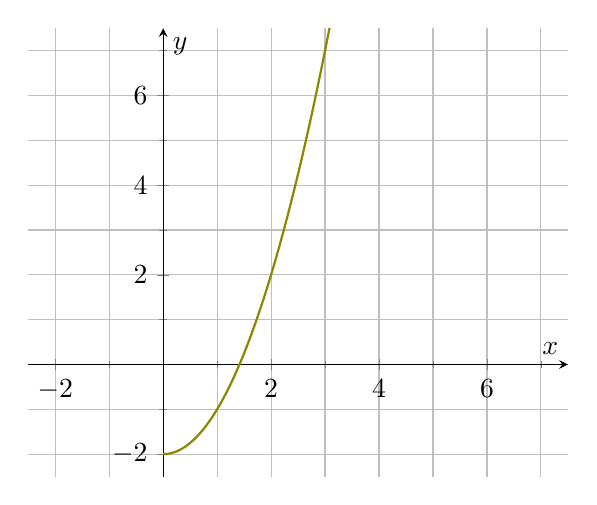
\begin{tikzpicture}
	\begin{axis}[
	axis lines = center, 
	xmin = -2.5, xmax = 7.5,
	ymin = -2.5, ymax = 7.5,
	xlabel = $x$, 
	ylabel = $y$,
	xtick = {-4,-2,...,6,8},
	ytick = {-4,-2,...,6,8},
	minor tick num = 1,
	grid = both,
	]
		\addplot[color = olive, thick, samples = 500, domain = 0:10] {x^2-2};
	\end{axis}
	\end{tikzpicture}
	}
\end{center}
\begin{enumerate}[label=\roman*)]
	\item Bestem $f^{-1}(-2)$.
	\item Løs ligningen $f(x) = 7$.
	\item Løs ligningen $f^{-1}(x) = 2$.
\end{enumerate}

\subsection*{Opgave 4}
Den inverse $f^{-1}$ til en funktion $f$ er givet ved følgende graf. 
\begin{center}
\resizebox{0.45\textwidth}{!}{
	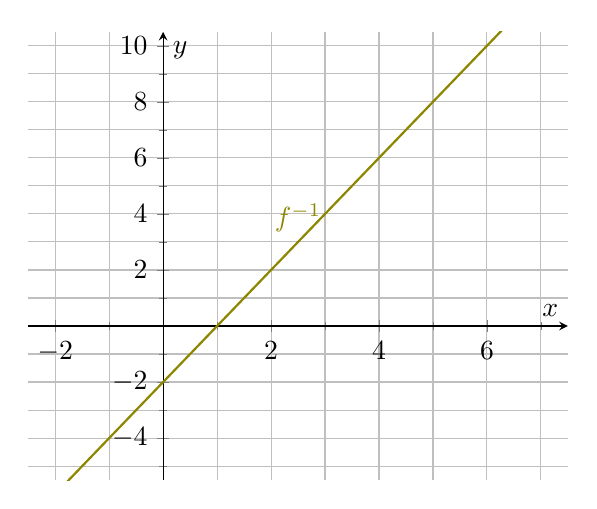
\begin{tikzpicture}
	\begin{axis}[
	axis lines = center, 
	xmin = -2.5, xmax = 7.5,
	ymin = -5.5, ymax = 10.5,
	xlabel = $x$, 
	ylabel = $y$,
	xtick = {-4,-2,...,6,8},
	ytick = {-8,-6,...,10,12},
	minor tick num = 1,
	grid = both,
	]
		\addplot[color = olive, thick, samples = 500, domain = -10:10] {2*x-2};
		\node[color = olive, anchor = south] at (axis cs: 2.5,3) {$f^{-1}$};
	\end{axis}
	\end{tikzpicture}
	}
\end{center}
\begin{enumerate}[label=\roman*)]
	\item Bestem $f^{-1}(1)$.
	\item Bestem $f(4)$.
	\item Løs ligningen $f^{-1}(x) = 8$.
	\item Løs ligningen $f(x) = 4$.
\end{enumerate}

\subsection*{Opgave 5}
\begin{enumerate}[label=\roman*)]
	\item Afgør om funktionerne $f$ og $g$ givet ved henholdsvis 
	\begin{align*}
		f(x) &= 2x - 4, \\
		g(x) &= \frac{x+4}{2}
	\end{align*}
	er hinandens inverse. 
	\item Afgør, om $f$ givet ved
	\begin{align*}
		f(x) = -x + 7
	\end{align*}
	er sin egen inverse.
	\item Afgør, om funktionerne $f$ og $g$ givet ved henholdsvis
	\begin{align*}
		f(x) &= 7^{x-9}\\
		g(x) &= \log_7(x)+8
	\end{align*}
	er hinandens inverse
	\item Afgør, om funktionerne $f$ og $g$ givet ved henholdsvis
	\begin{align*}
		f(x) &= \sqrt[5]{2x+4},\\
		g(x) &= \frac{y^5-4}{4}
	\end{align*}
	er hinandens inverse
	\item Afgør, om funktionerne $f$ og $g$ givet ved henholdsvis
	\begin{align*}
		f(x) &= 6^{2x^9 - 4} \\
		g(x) &= \sqrt[9]{\frac{\log_6(x) + 4}{2}}
	\end{align*}
	er hinandens inverse.
	
\end{enumerate}

\subsection*{Opgave 6}
\begin{enumerate}[label=\roman*)]
	\item Bestem en invers funktion til funktionen $f$ givet ved
	\begin{align*}
		f(x) = -10x + 7
	\end{align*}
	\item Bestem en invers funktion til funktionen $f$ givet ved
	\begin{align*}
		f(x) = -x-2
	\end{align*}
	\item Bestem en invers funktion til funktionen $f$ givet ved
	\begin{align*}
		f(x) = (x-5)^3 + 1
	\end{align*}
	\item Bestem en invers funktion til funktionen $f$ givet ved
	\begin{align*}
		f(x) = 2^{9x-10}
	\end{align*}
	\item Bestem en invers funktion til funktionen $f$ givet ved
	\begin{align*}
		f(x) = \sqrt{2x -3}
	\end{align*}
	\item Bestem en invers funktion til funktionen $f$ givet ved
	\begin{align*}
		f(x) = \log_7(5x^3-6)
	\end{align*}
\end{enumerate}

\subsection*{Opgave 7}
Overvej, hvordan grafen for en funktion skal se ud, hvis den skal være sin egen inverse funktion. Kan du give eksempler på funktioner, der er deres egne inverse?

\subsection*{Opgave 8 (Svær)}
Prøv at give et bevis for, at en funktion er bijektiv hvis og kun hvis den har en invers funktion. Antag først, at funktionen er bijektiv og vis derefter, at den har en invers funktion. Antag efterfølgende, at funktionen har en invers funktion og brug dette til at vise, at funktionen er bijektiv. 

